\documentclass[12pt]{article}
\usepackage{xeCJK}

\usepackage{listings}
\usepackage{xcolor}

\usepackage[a4paper, left=3.17cm, right=3.17cm, top=2.54cm, bottom=2.54cm]{geometry}
\usepackage{fancyhdr} % header and footer
\usepackage[T1]{fontenc}
\usepackage{mathptmx}
\usepackage{amsmath}
\usepackage{amsfonts}
\usepackage{chemformula}
\usepackage{cite}
\usepackage[colorlinks, linkcolor=black, anchorcolor=black, citecolor=black]{hyperref}
\usepackage{graphicx}
\usepackage{hyperref}

\setCJKmainfont{Songti SC}
\setCJKsansfont{Songti SC}
\setCJKmonofont{Songti SC}

\lstset{ %
  language=C++,
  backgroundcolor=\color{black!5},
  basicstyle=\footnotesize,
}
% show paragraphs in table of contentes
\setcounter{tocdepth}{4}
\setcounter{secnumdepth}{4}

\setlength{\parskip}{0.5em}
\title{C语言词法分析程序的设计与实现}
\author{\textup{吴清柳}}
\begin{document}
\begin{titlepage}
    \newcommand{\HRule}{\rule{\linewidth}{0.5mm}}
    
\includegraphics[width=8cm]{title/logo_bupt.png}\\[1cm]
    \center
    \quad\\[1.5cm]
    \textsl{\Large 北京邮电大学}\\[0.5cm]
    \textsl{\large  计算机学院}\\[0.5cm]
    \makeatletter
    \HRule \\[0.4cm]
    {\huge \bfseries \@title}\\[0.4cm]
    \HRule \\[1.5cm]
    % \begin{minipage}{0.4\textwidth}
    %     \begin{flushleft} \large
    %         \emph{Author:}\\
    %         \@author
    %     \end{flushleft}
    % \end{minipage}
    % ~
    % \begin{minipage}{0.4\textwidth}
    %     \begin{flushright} \large
    %         \emph{Supervisor:} \\
    %         \textup{ 王雅文}
    %     \end{flushright}
    % \end{minipage}\\[3cm]
    \makeatother
    {\large (C++版和FLEX版均实现)}\\[0.5cm]
    {\large 姓名: 吴清柳}\\[0.5cm]
    {\large 学号: 2020211597}\\[0.5cm]
    {\large 班级: 2020211323}\\[0.5cm]
    {\large 指导老师: 王雅文}\\[0.5cm]
    {\large \emph{课程名称: 编译原理}}\\[0.5cm]
    {\large \today}\\[2cm]
    \vfill
\end{titlepage}

\tableofcontents
\newpage

% set page stype to fancy then decorate it
\pagestyle{fancy}
\fancyhead{} % clear all header fields
\fancyhead[LE, RO]{吴清柳 2020211597}
\fancyhead[LO, RE]{C语言词法分析程序的设计与实现}
\fancyfoot{} % clear all footer fileds
\fancyfoot[CE, CO]{\thepage}

\section{题目及要求}
\begin{enumerate}
  \item 设计一个C语言词法分析程序;
  \item 可以识别出用C语言编写的源程序中的每个单词符号, 运算符, 数字, 字符(包括转义字符)等,
  并以<记号, 属性>的形式 输出每个单词符号;
  \item 可以识别并跳过源程序中的注释;
  \item 可以统计源程序中的语句行数, 各类单词个数, 字符总数, 并输出统计结果;
  \item 可以识别C语言程序源代码中存在的词法错误, 并报告错误出现的位置;
  \item 对源程序中出现的错误进行适当的恢复, 让词法分析可以继续进行;
  \item 对源程序进行一次扫描, 即可检查并报告源程序中存在的所有词法错误, 并输出
  源程序中所有的记号.
\end{enumerate}

\section{实验设备}
Ubuntu 20.04.5 LTS on Windows 10 x86\_64, \\[0.5cm]
macOS 12.6 21G115 arm64, \\[0.5cm]
Neovim v0.7.2, \\[0.5cm]
clang-1400.0.29.102, \\[0.5cm]
flex 2.6.4 \\[0.5cm]

\section{程序设计说明}
\begin{enumerate}
\item 词法分析程序的作用:
  \begin{enumerate}
  \item 扫描源程序字符流;
  \item 按照源语言的词法规则识别出各类单词符号;
  \item 产生用于语法分析的记号序列;
  \item 词法检查;
  \item 创建符号表, 将识别出来的标识符放入符号表中;
  \item 跳过源程序中的注释和空格等, 把错误信息和源代码联系起来;
  \end{enumerate}
\item 源程序代词类别:
  \begin{enumerate}
    \item 关键字;
    \item 用户定义变量标识符;
    \item 数字, 字符和字符串常量;
    \item 运算符;
    \item 分隔符;
  \end{enumerate}
\item 设计思路:
  利用有限状态自动机模型, 将整个源代码分析的过程转化为不同状态之间的转移, 在画好
  状态转移图之后, 借用C++的switch语句或if/else语句将状态转移图描述出来. 此外, 
  实现好读取源代码, 缓冲区, 以及输出分析结果, 和将常量和变量名插入到符号表的功能.
\item 伪代码描述:
\begin{lstlisting}
// Initializing...
while(End of source file not reached) {
  ch = getchar();
  switch(ch) {
    determine state based on the input char
    case 0:
    ...
  }
  switch(State) {
    // Limited state machine process
    case 0:
      // state 0 process
    case 1:
      // state 1 process
    ...
  }
}
\end{lstlisting}
\end{enumerate}

\section{实验流程图}
\begin{figure}
  \begin{center}
    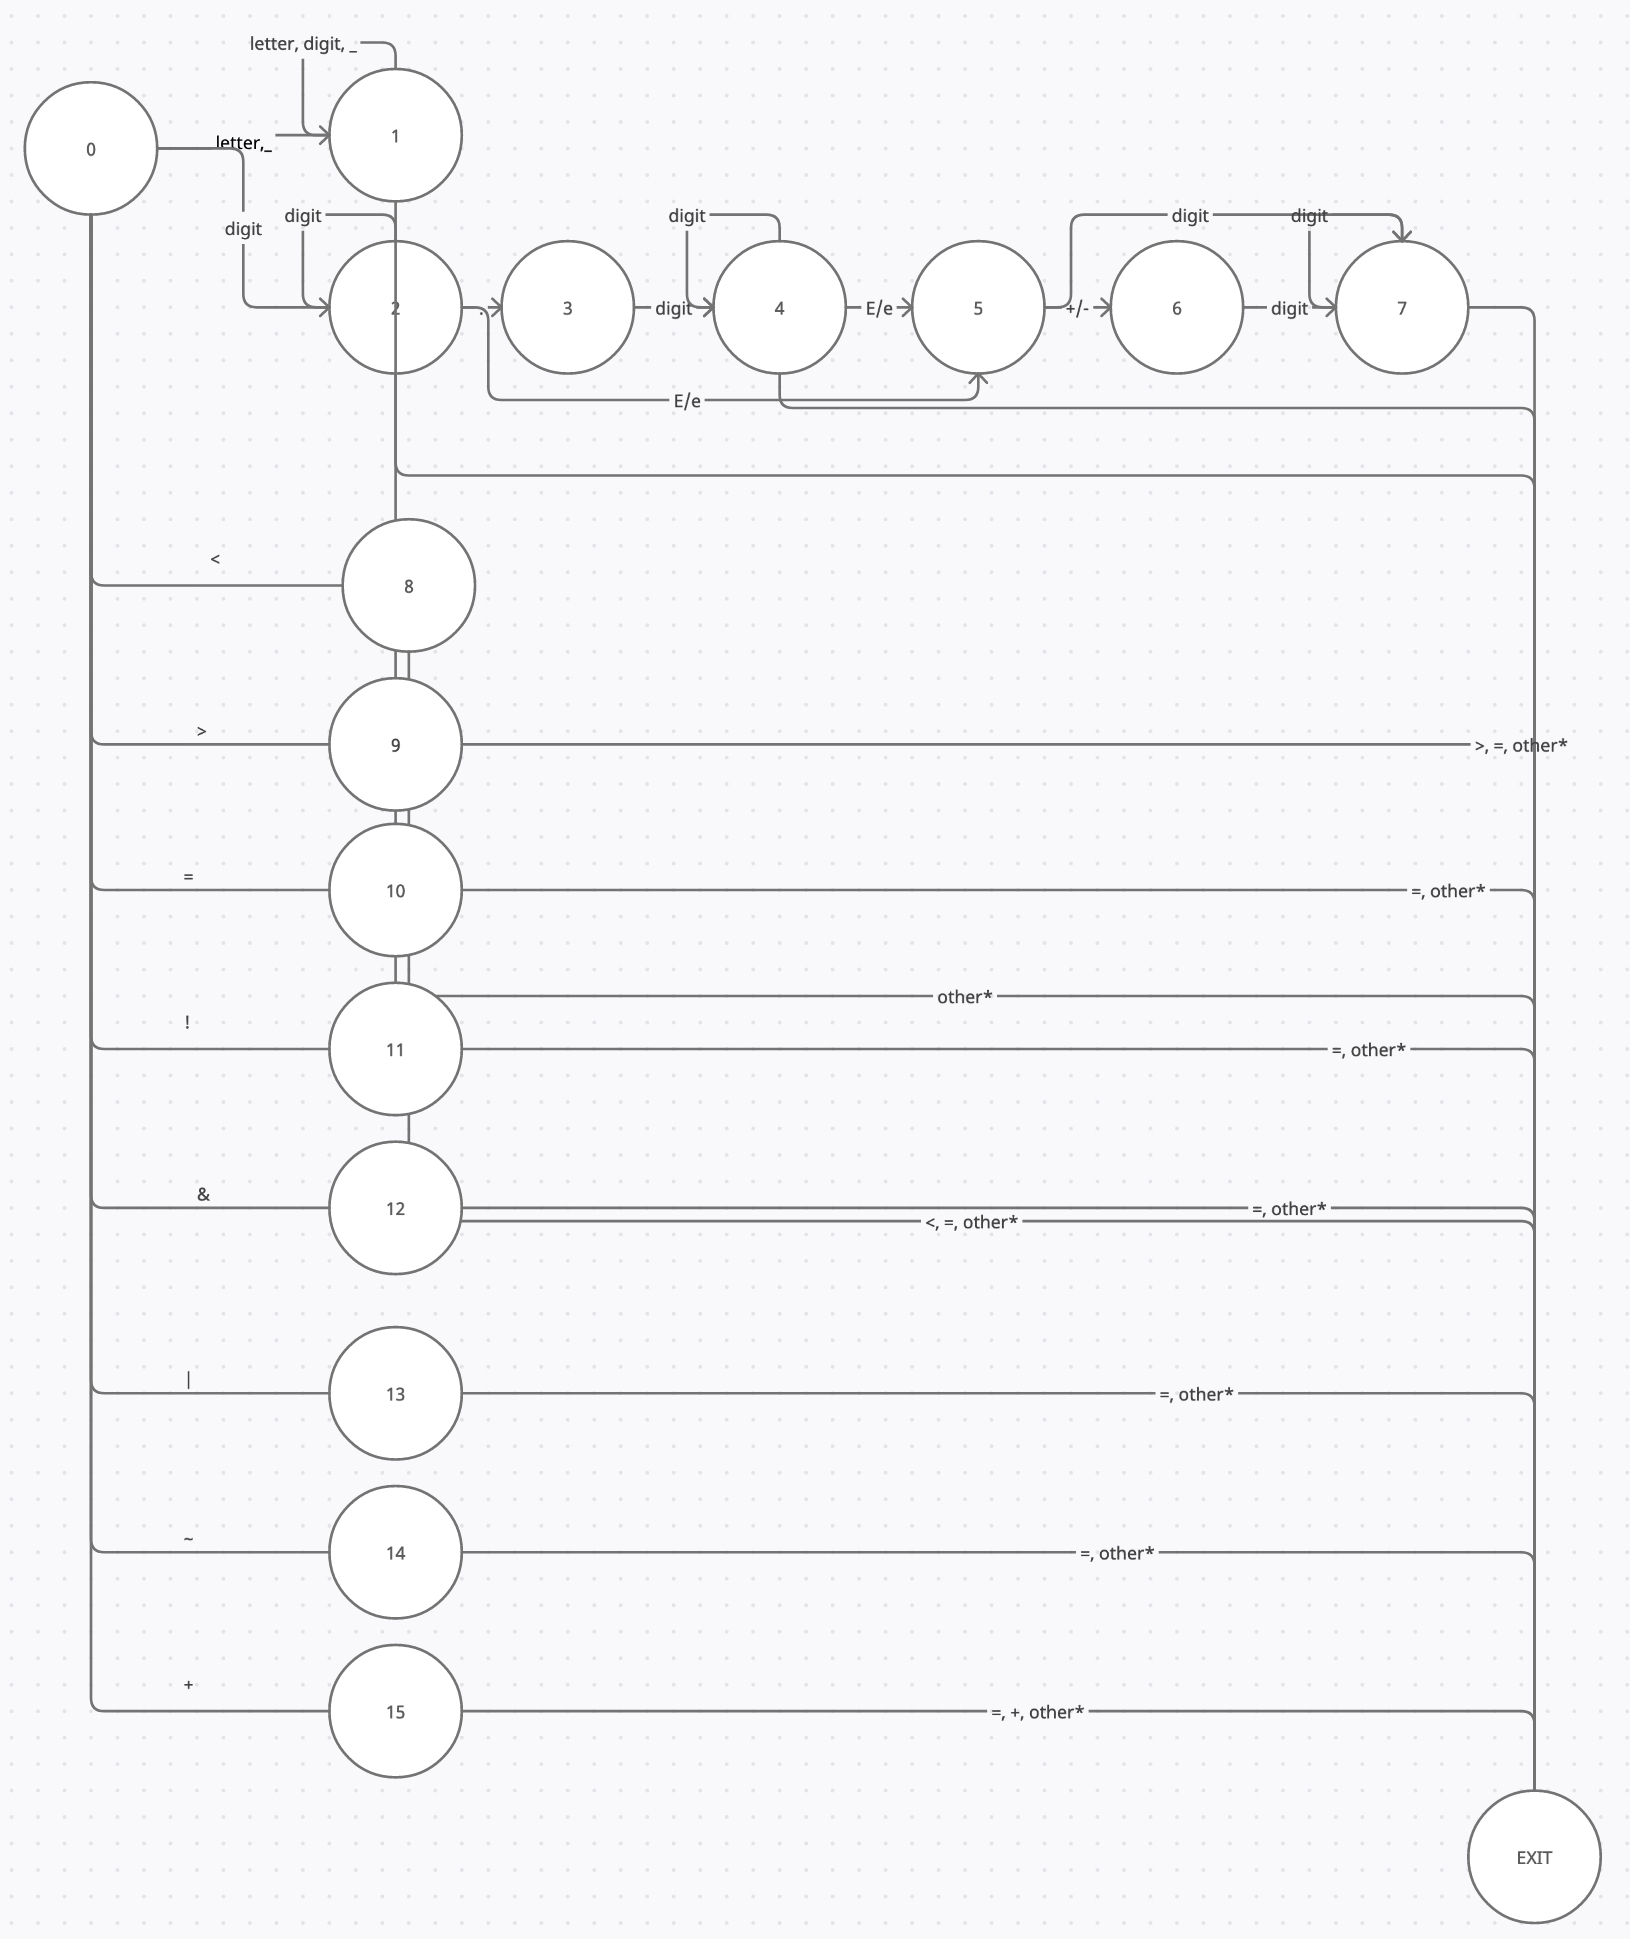
\includegraphics[width=0.95\textwidth]{figures/Page0.png}
  \end{center}
  \caption{词法分析程序的状态转移图 1}
  \label{fig:StateFig1}
\end{figure}

\begin{figure}
  \begin{center}
    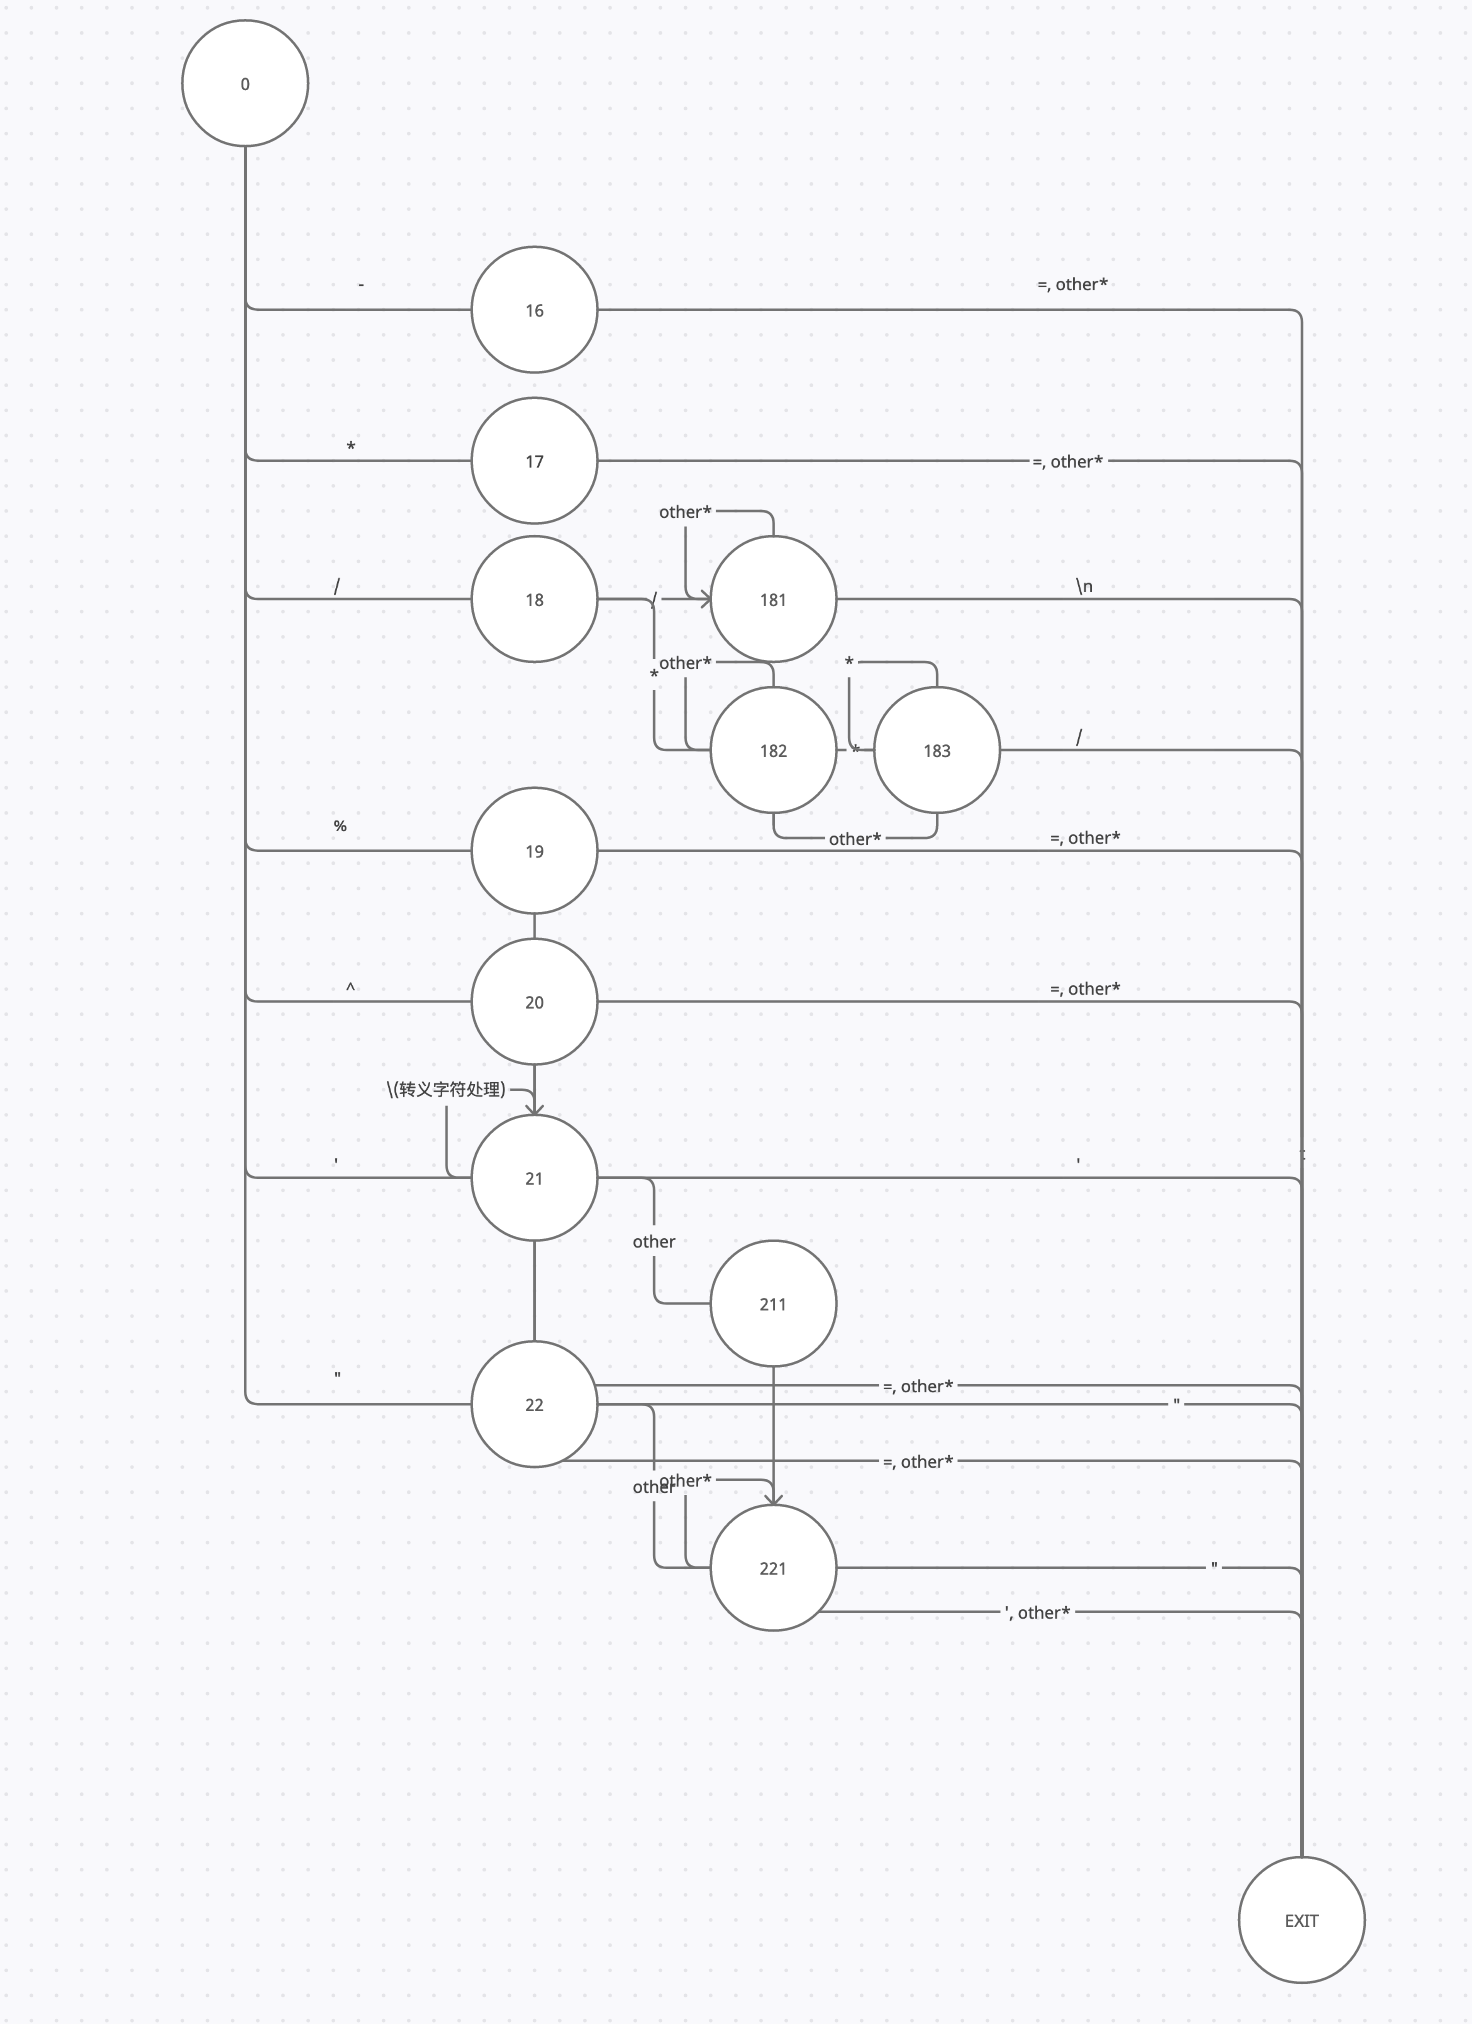
\includegraphics[width=0.95\textwidth]{figures/Page1.png}
  \end{center}
  \caption{词法分析程序的状态转移图 2}
  \label{fig:StateFig2}
\end{figure}
用状态转移图描述的词法分析程序如下图~\ref{fig:StateFig1}和图~\ref{fig:StateFig2}. \\
其中状态0是起始状态, 状态EXIT为当源代码文件未分析完毕时回到状态0, 分析完毕时退出.

\section{实验程序}
\subsection{C++版本}
出于模块化, 解耦合, 可扩展性和可读性考虑, 将词法分析程序划分为\textbf{符号和符号表}
与\textbf{词法分析处理和输入输出}两个模块, 分别在 Symbol.h, Symbol.cpp, Lex.h和Lex.cpp
四个源代码文件中进行实现, 并使用CMake作为构建工具.

其中, Symbol.h和Symbol.cpp对记号(Symbol)及记号表(SymbolList)的类进行成员和方法定义和实现,
 Lex.h和Lex.cpp对词法分析处理, 输入和输出类Lex进行成员和方法定义和实现.

main.cpp承担着作为词法分析程序入口的功能.

\subsubsection{main.cpp}
词法分析程序入口
\lstinputlisting{../src/main.cpp}
\subsubsection{Symbol.h}
对记号(Symbol)及记号表(SymbolList)的类成员和方法定义;
\lstinputlisting{../src/Symbol.h}
\subsubsection{Symbol.cpp}
对记号(Symbol)及记号表(SymbolList)的类成员和方法实现;
\lstinputlisting{../src/Symbol.cpp}
\subsubsection{Lex.h}
词法分析处理和输出类Lex的成员和方法定义;
\lstinputlisting{../src/Lex.h}
\subsubsection{Lex.cpp}
词法分析处理和输出类Lex的成员和方法实现;
\lstinputlisting{../src/Lex.cpp}

\subsection{FLEX版本}
在C++版本实现思路的基础上, 通过学习FLEX的语法, 用FLEX实现了相同功能的版本.
\subsubsection{FLEX介绍}
\paragraph{基本结构}
一个FLEX程序的基本结构为
\begin{lstlisting}
Statements/Definitaions
%%
Rules
%%
User Functions(optional)
\end{lstlisting}
我们将lexer保存在扩展名为.i的文件中.

\paragraph{Definitions}
我们可以为工具添加如下\textbf{options}:
\begin{itemize}
  \item \%option noyywrap -> flex将只读一个输入文件
  \item \%option case-insensitive -> flex将不区分大小写
\end{itemize}
我们也可以对某些正则表达式设置\textbf{start states}: \\
\begin{lstlisting}
%x STATE_NAME
\end{lstlisting}
对于多行注释, 这是很好用的, 因为当到达注释末尾的时候, 可以更方便的搜索连续的内容
并结束注释状态. \\
此外, 我们可以利用正则表达式定义一些\textbf{Identifiers}并给他们命名, 如: \\
\begin{lstlisting}
print [ -\~] // space to \~(所有可打印的ASCII字符)
\end{lstlisting}
语句识别\{print\}作为一个包含所有可打印字符的group. \\
使用identifiers我们可以在匹配特定token的时候方便的使用名称调用, 而不是每次都要
书写完整的正则表达式. \\
最后, 我们也可以定义一个\textbf{literal block of code}, 即事实上的c代码, 并且可以
包含头文件, 常量, 全局变量和函数定义等. 这些代码将会被复制到flex生成的分析器中, 
并最终成为编译器的一部分. \\
要定义一个这样的block, 要以如下形式:
\begin{lstlisting}
%{
  // literal c code
%}
\end{lstlisting}

\paragraph{Rules}
我们在这里定义tokens的规则.
我们使用这样的格式: \\
\begin{lstlisting}
regex-rule { // c action-code }
\end{lstlisting}
左边部分仅包含正则表达式规则, 而右边部分是定义了行为的实际上的c代码. 目前我们将
仅仅输出到标准输出说我们找到了一个特定的token, 在那之后我们会返回token的记号和属性.

所以, 要搜索一个可打印字符串序列, 我们可能会使用: \\
\begin{lstlisting}
{print}+ { printf("Found printable character sequence %s\n", yytext); }
\end{lstlisting}
左边是一条匹配包含至少一个可打印字符的字符串的正则表达式规则, 变量yytext
包含每次识别到的token.

\paragraph{User Functions}
最后, 在FLEX中我们也可以定义函数. \\
例如, 代码可以包含主程序入口main(), 也可以包含一个错误信息打印函数yyerror().
yywrap()函数由option "\%option noyywrap"定义. 我们可能还需要一个打印token的记号和
属性的函数, 比如ret\_print(), 将token传入到后面的处理程序, 如语法分析程序, 并同时
输出到标准输出.

\paragraph{Variables}
Flex的变量有如下几种:
\begin{itemize}
  \item char *yytext -> 包含识别到的token;
  \item int yyleng -> 包含识别到的token的长度;
  \item YYSTYPE yylval -> 用来和之后的程序, 例如语法分析程序通信.
\end{itemize}

\paragraph{Usage of Flex}
要使用Flex, 需要先安装Flex, 之后执行以下命令: \\[0.5cm]
flex lex.l // lex.l is the flex file \\[0.5cm]
clang lex.yy.c -o c\_lex -lfl // or use gcc instead, generate c source file \\[0.5cm]
./lex input\_file // lex will take input\_file as c source file to be analysed \\[0.5cm]
默认情况下, 分析结果将输出到console中.

\subsubsection{FLEX源代码清单}
\begin{lstlisting}
// lex.i
\end{lstlisting}
\lstinputlisting{../lex.i}

\section{实验输入(测试程序)}
\subsubsection{测试样例1}
\lstinputlisting{../build/sin_1}
\subsubsection{测试样例2}
\lstinputlisting{../build/sin_2}

\section{实验运行结果及分析说明}
\subsection{输出格式概述}
\begin{itemize}
  \item 在Statistic information之前的是输入词法分析程序的源代码文件中解析到的符号, 格式为
L[行号]: <[记号], [属性]>.
  \item Statistic information(统计信息)有如下格式:
  \begin{itemize}
    \item 第一行为行数, 字符数和符号数统计, 格式为[行数] lines, [字符数] characters,
    [符号数] symbols;
    \item 之后跟[符号数]行, 每行是一个符号及其出现次数, 格式为<[记号], [属性]> appeared
     [出现次数] times;
  \end{itemize}
\end{itemize}

\subsection{测试样例1的输出}
测试样例1为较简短的样例, 用于进行输入输出功能和状态转移基本功能的测试;
\subsubsection{C++版词法分析程序测试}
\lstinputlisting{code_lists/sin_1_output}
\subsubsection{FLEX版词法分析程序测试}
\lstinputlisting{code_lists/sin_1_flex}
\subsection{测试样例2的输出}
测试样例2为较长, 测试内容较全面的样例, 用于对词法分析程序实现的各项功能进行测试.
\subsubsection{C++版词法分析程序测试}
\lstinputlisting{code_lists/sin_2_output}
\subsubsection{FLEX版词法分析程序测试}
\lstinputlisting{code_lists/sin_2_flex}
\subsection{分析和总结}
通过C++版和FLEX版分析结果的对照, 说明该C语言词法分析程序有以下功能:
\begin{enumerate}
  \item 可以识别出用C语言编写的源程序中的每个单词符号, 运算符, 数字等,
  并以<记号, 属性>的形式 输出每个单词符号, 包括转义字符;
  \item 可以识别并跳过源程序中的注释;
  \item 可以统计源程序中的语句行数, 各类单词个数, 字符总数, 并输出统计结果;
  \item 可以识别C语言程序源代码中存在的词法错误, 并报告错误出现的位置;
  \item 对源程序中出现的错误进行适当的恢复, 让词法分析可以继续进行;
  \item 对源程序进行一次扫描, 即可检查并报告源程序中存在的所有词法错误, 并输出
  源程序中所有的记号.
\end{enumerate}

\section{心得体会}
通过这次词法分析程序的上手实践, 让我对编译原理课程的认识增加了除理论知识之外的内容, 
亲自动手实现词法分析程序也让我对编译器进行词法分析的过程有了更加深入的理解. 

词法分析程序与语法分析程序之间的关系可以有3种, 分别是词法分析程序作为独立的
一遍, 词法分析程序作为语法分析程序的子程序, 和词法分析程序和语法分析程序作为
协同程序. 在本次课程设计中, 将词法分析程序作为了独立的一遍, 可以将词法分析程序
的输出放入到单独的中间文件, 让之后的语法分析程序读取中间文件即可获得词法分析
结果, 有利于提柜编译程序的效率.

此外, 通过本次课程设计, 通过自己的动手亲身体验了将词法分析和语法分析等过程独立
处理的好处: 如可以将各部分需要实现的功能进行良好封装和解耦合, 对外只暴露接口和
提供服务, 各模块的具体实现对外部不可见, 简化了各部分实现的时候需要考虑的内容, 
从而在实现识别并去除空格, 注释等功能的时候思路更加清晰, 还可以让程序可移植性, 
可扩展性更强.

再次, 在本次课程设计中我还尝试了利用FLEX自动生成词法分析程序, 在FLEX自动生成版本
和自己书写的版本的对比中, 体会到了FLEX功能的强大, 灵活和便利, 令我受益匪浅.

总体来说, 在本次课程设计过程中, 我对上学期所学形式语言和自动机知识, 以及本学期
所学的词法分析内容都有了更加深刻的理解, 并掌握了运用方法; 此外, 编程能力, 程序
设计能力等也有了不小的提升.

\section{附录}
代码仓库: \href{https://github.com/Micuks/Lexical\_Analysis}{Micuks/Lexical\_Analysis}

% \bibliographystyle{ieeetrans}
% \bibliography{Assignment_Ref}

\end{document}
